\newpage
\section*{\centerline{Список литературы}}
\vspace{1cm}
 \paragraph{1} https://askubuntu.com\\

 \paragraph{2} https://unix.stackexchange.com\\
 
 \paragraph{3} https://http://www.rhd.ru/docs/manuals/enterprise/RHEL-AS-2.1-Manual/\\
 
 \paragraph{4} https://stackoverflow.com/ \\
 
 \paragraph{5} http://www.hrono.info/biograf/bio\_ l/lermontov\_ mu.php
 \\
 
 \newpage
 \section*{\centerline{Вывод по работе}}
 \vspace{1cm}
 В качестве выводов можно выделить следующие компоненты:\\
 1) Были изучены и использованы команды для работы с архивами (архивирование, распаковка, просмотр списка файлов в архиве) \\
 2) Также получены навыки необходимые для скачивания файлов со сторонних ресурсов \\

 3) Были изучены команды и ключи, с помощью которых можно осуществлять поиск файлов/строк/слов/символов и их изменение. \\
 4) Далее мы научились узнавать и отображать типы файлов и их содержимое \\
 5) Просмотрены и использованы команды, изменяющие и отображающие права файлов и директорий \\
 6) Изучены и применены команды, необходимые для ввода и вывода информации из файла \\
 \begin{center}
		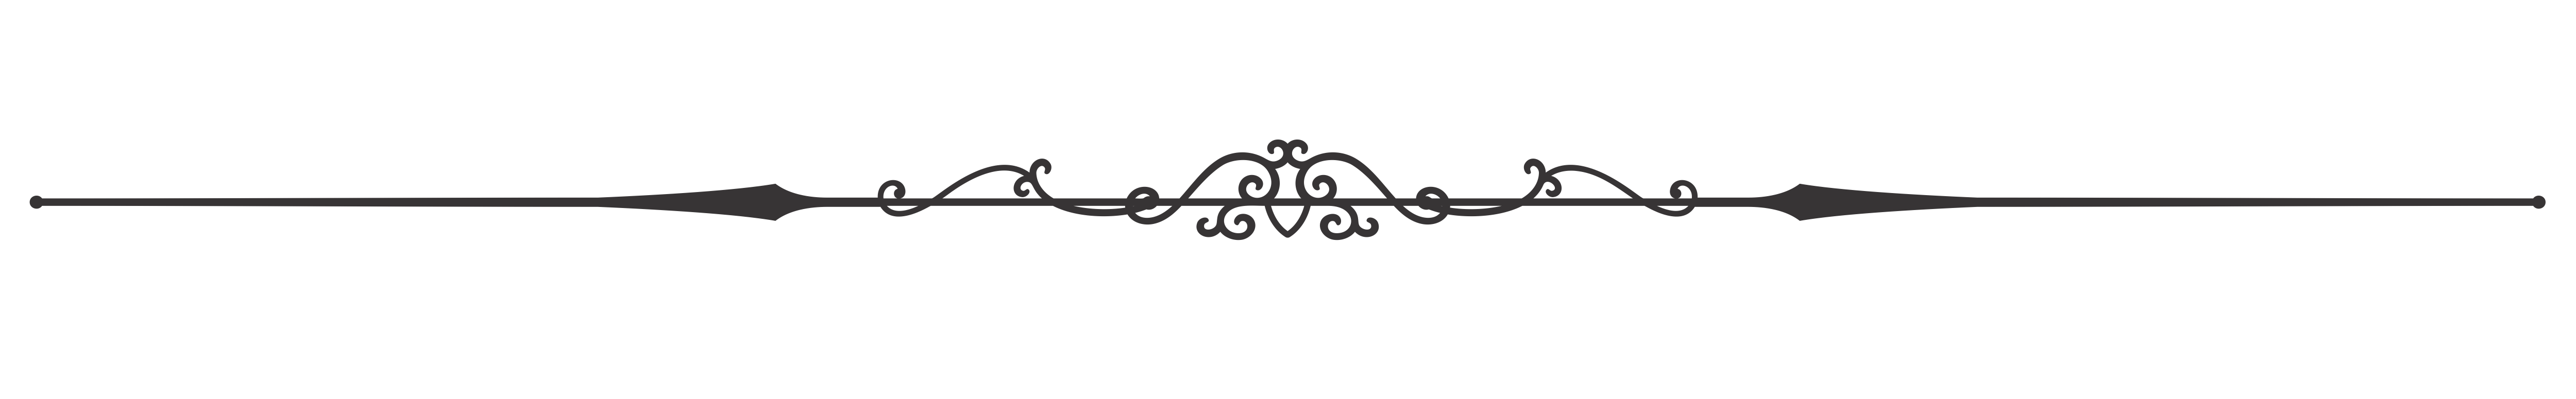
\includegraphics[width=0.8\textwidth]{line.png}
	\end{center}

 \vspace{1.5cm}
 \centerline{Спасибо за внимание}

)